\documentclass{standalone}
\usepackage{tikz}
\usetikzlibrary{patterns, positioning}


\begin{document}
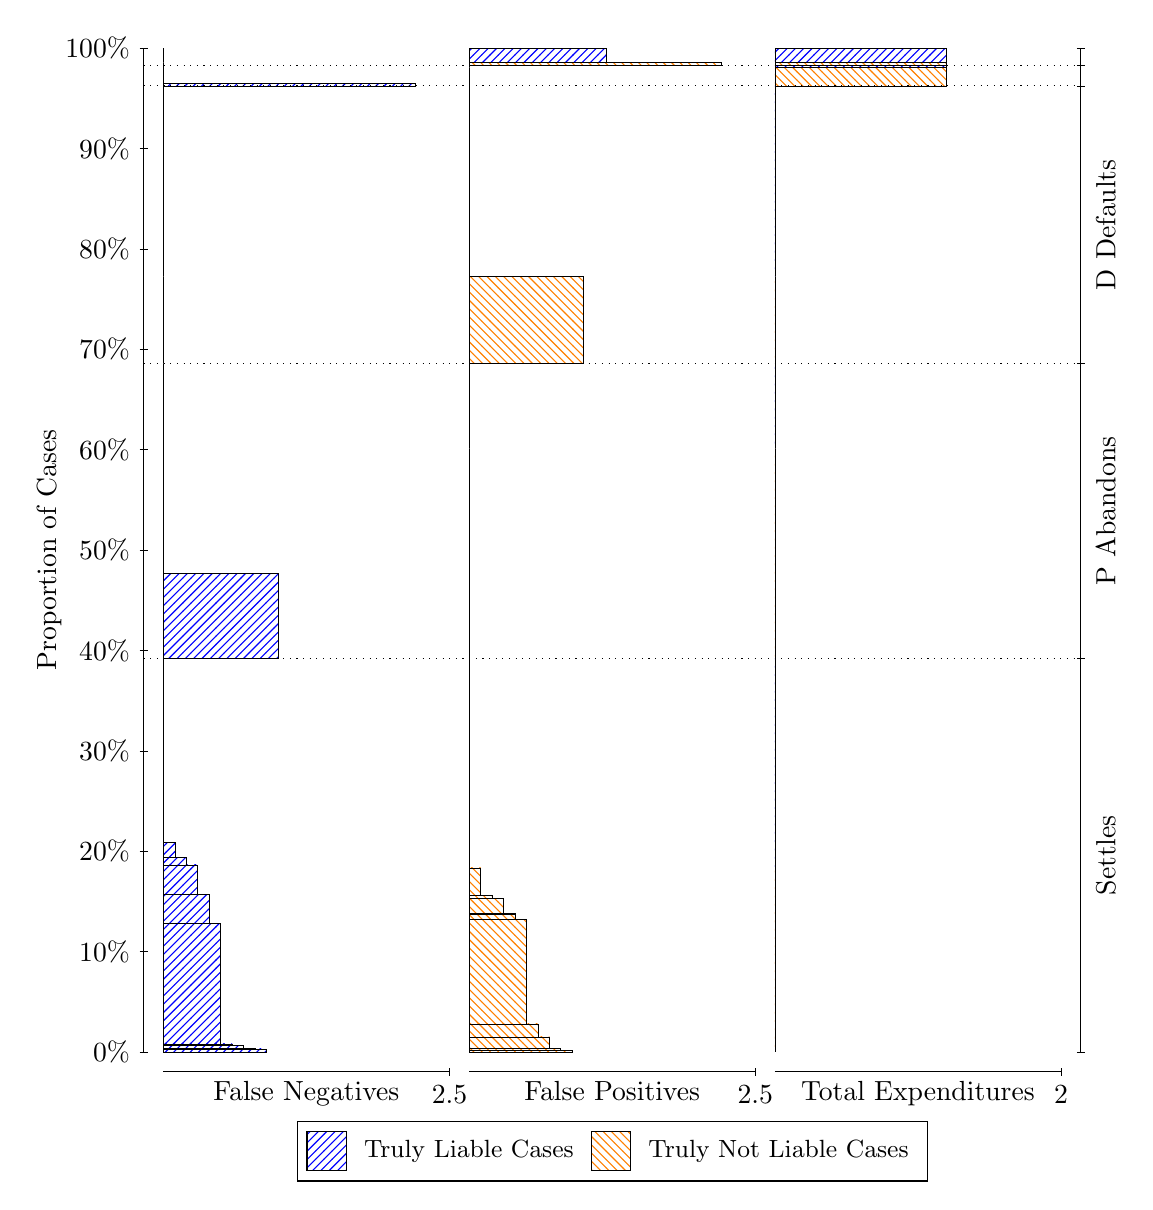
\begin{tikzpicture}
\draw[black, very thin] (1.5,1.75) -- (1.5,14.5);
\node[rotate=90, text=black, anchor=center] at (0.3, 8.125) {Proportion of Cases};
\draw[black, very thin] (1.45,1.75) -- (1.55,1.75);
\node[text=black, anchor=east] at (1.45, 1.75) {0\%};
\draw[black, very thin] (1.45,3.025) -- (1.55,3.025);
\node[text=black, anchor=east] at (1.45, 3.025) {10\%};
\draw[black, very thin] (1.45,4.3) -- (1.55,4.3);
\node[text=black, anchor=east] at (1.45, 4.3) {20\%};
\draw[black, very thin] (1.45,5.575) -- (1.55,5.575);
\node[text=black, anchor=east] at (1.45, 5.575) {30\%};
\draw[black, very thin] (1.45,6.85) -- (1.55,6.85);
\node[text=black, anchor=east] at (1.45, 6.85) {40\%};
\draw[black, very thin] (1.45,8.125) -- (1.55,8.125);
\node[text=black, anchor=east] at (1.45, 8.125) {50\%};
\draw[black, very thin] (1.45,9.4) -- (1.55,9.4);
\node[text=black, anchor=east] at (1.45, 9.4) {60\%};
\draw[black, very thin] (1.45,10.675) -- (1.55,10.675);
\node[text=black, anchor=east] at (1.45, 10.675) {70\%};
\draw[black, very thin] (1.45,11.95) -- (1.55,11.95);
\node[text=black, anchor=east] at (1.45, 11.95) {80\%};
\draw[black, very thin] (1.45,13.225) -- (1.55,13.225);
\node[text=black, anchor=east] at (1.45, 13.225) {90\%};
\draw[black, very thin] (1.45,14.5) -- (1.55,14.5);
\node[text=black, anchor=east] at (1.45, 14.5) {100\%};

\draw[black, very thin] (13.4,1.75) -- (13.4,14.5);
\draw[black, very thin] (13.35,1.75) -- (13.45,1.75);
\node[anchor=west] at (13.35, 1.75) {};
\draw[black, very thin] (13.35,6.7457) -- (13.45,6.7457);
\node[anchor=west] at (13.35, 6.7457) {};
\draw[black, very thin] (13.35,10.493) -- (13.45,10.493);
\node[anchor=west] at (13.35, 10.493) {};
\draw[black, very thin] (13.35,14.019) -- (13.45,14.019);
\node[anchor=west] at (13.35, 14.019) {};
\draw[black, very thin] (13.35,14.283) -- (13.45,14.283);
\node[anchor=west] at (13.35, 14.283) {};
\draw[black, very thin] (13.35,14.5) -- (13.45,14.5);
\node[anchor=west] at (13.35, 14.5) {};

\draw[black, very thin, pattern color=blue, pattern=north east lines] (1.75,1.75) rectangle (3.058,1.7885);
\draw[black, very thin, pattern color=blue, pattern=north east lines] (1.75,1.7885) rectangle (2.9127,1.7925);
\draw[black, very thin, pattern color=blue, pattern=north east lines] (1.75,1.7925) rectangle (2.7673,1.8344);
\draw[black, very thin, pattern color=blue, pattern=north east lines] (1.75,1.8344) rectangle (2.622,1.8407);
\draw[black, very thin, pattern color=blue, pattern=north east lines] (1.75,1.8407) rectangle (2.622,1.8536);
\draw[black, very thin, pattern color=blue, pattern=north east lines] (1.75,1.8536) rectangle (2.4767,3.3793);
\draw[black, very thin, pattern color=blue, pattern=north east lines] (1.75,3.3793) rectangle (2.3313,3.7526);
\draw[black, very thin, pattern color=blue, pattern=north east lines] (1.75,3.7526) rectangle (2.186,4.1256);
\draw[black, very thin, pattern color=blue, pattern=north east lines] (1.75,4.1256) rectangle (2.0407,4.221);
\draw[black, very thin, pattern color=blue, pattern=north east lines] (1.75,4.221) rectangle (1.8953,4.4091);
\draw[black, very thin, pattern color=orange, pattern=north west lines] (1.75,4.4091) rectangle (1.75,6.7457);
\draw[black, very thin, pattern color=blue, pattern=north east lines] (1.75,6.7457) rectangle (3.2033,7.8264);
\draw[black, very thin, pattern color=orange, pattern=north west lines] (1.75,7.8264) rectangle (1.75,10.493);
\draw[black, very thin, pattern color=orange, pattern=north west lines] (1.75,10.493) rectangle (1.75,11.601);
\draw[black, very thin, pattern color=blue, pattern=north east lines] (1.75,11.601) rectangle (1.75,14.019);
\draw[black, very thin, pattern color=blue, pattern=north east lines] (1.75,14.019) rectangle (4.9473,14.052);
\draw[black, very thin, pattern color=orange, pattern=north west lines] (1.75,14.052) rectangle (1.75,14.283);
\draw[black, very thin, pattern color=orange, pattern=north west lines] (1.75,14.283) rectangle (1.75,14.315);
\draw[black, very thin, pattern color=blue, pattern=north east lines] (1.75,14.315) rectangle (1.75,14.5);
\draw[black, very thin, pattern color=orange, pattern=north west lines] (5.6333,1.75) rectangle (6.9413,1.7668);
\draw[black, very thin, pattern color=orange, pattern=north west lines] (5.6333,1.7668) rectangle (6.796,1.7964);
\draw[black, very thin, pattern color=orange, pattern=north west lines] (5.6333,1.7964) rectangle (6.6507,1.9403);
\draw[black, very thin, pattern color=orange, pattern=north west lines] (5.6333,1.9403) rectangle (6.5053,2.1081);
\draw[black, very thin, pattern color=orange, pattern=north west lines] (5.6333,2.1081) rectangle (6.36,3.4381);
\draw[black, very thin, pattern color=orange, pattern=north west lines] (5.6333,3.4381) rectangle (6.2147,3.4985);
\draw[black, very thin, pattern color=orange, pattern=north west lines] (5.6333,3.4985) rectangle (6.2147,3.513);
\draw[black, very thin, pattern color=orange, pattern=north west lines] (5.6333,3.513) rectangle (6.0693,3.6985);
\draw[black, very thin, pattern color=orange, pattern=north west lines] (5.6333,3.6985) rectangle (5.924,3.7411);
\draw[black, very thin, pattern color=orange, pattern=north west lines] (5.6333,3.7411) rectangle (5.7787,4.0866);
\draw[black, very thin, pattern color=blue, pattern=north east lines] (5.6333,4.0866) rectangle (5.6333,6.7457);
\draw[black, very thin, pattern color=orange, pattern=north west lines] (5.6333,6.7457) rectangle (5.6333,9.4118);
\draw[black, very thin, pattern color=blue, pattern=north east lines] (5.6333,9.4118) rectangle (5.6333,10.493);
\draw[black, very thin, pattern color=orange, pattern=north west lines] (5.6333,10.493) rectangle (7.0867,11.601);
\draw[black, very thin, pattern color=blue, pattern=north east lines] (5.6333,11.601) rectangle (5.6333,14.019);
\draw[black, very thin, pattern color=orange, pattern=north west lines] (5.6333,14.019) rectangle (5.6333,14.251);
\draw[black, very thin, pattern color=blue, pattern=north east lines] (5.6333,14.251) rectangle (5.6333,14.283);
\draw[black, very thin, pattern color=orange, pattern=north west lines] (5.6333,14.283) rectangle (8.8307,14.315);
\draw[black, very thin, pattern color=blue, pattern=north east lines] (5.6333,14.315) rectangle (7.3773,14.5);
\draw[black, very thin, pattern color=orange, pattern=north west lines] (9.5167,1.75) rectangle (9.5167,4.0866);
\draw[black, very thin, pattern color=blue, pattern=north east lines] (9.5167,4.0866) rectangle (9.5167,6.7457);
\draw[black, very thin, pattern color=orange, pattern=north west lines] (9.5167,6.7457) rectangle (9.5167,9.4118);
\draw[black, very thin, pattern color=blue, pattern=north east lines] (9.5167,9.4118) rectangle (9.5167,10.493);
\draw[black, very thin, pattern color=orange, pattern=north west lines] (9.5167,10.493) rectangle (9.5167,11.601);
\draw[black, very thin, pattern color=blue, pattern=north east lines] (9.5167,11.601) rectangle (9.5167,14.019);
\draw[black, very thin, pattern color=orange, pattern=north west lines] (9.5167,14.019) rectangle (11.697,14.251);
\draw[black, very thin, pattern color=blue, pattern=north east lines] (9.5167,14.251) rectangle (11.697,14.283);
\draw[black, very thin, pattern color=orange, pattern=north west lines] (9.5167,14.283) rectangle (11.697,14.315);
\draw[black, very thin, pattern color=blue, pattern=north east lines] (9.5167,14.315) rectangle (11.697,14.5);
\draw[black, dotted] (1.5,6.7457) -- (13.4,6.7457);
\draw[black, dotted] (1.5,10.493) -- (13.4,10.493);
\draw[black, dotted] (1.5,14.019) -- (13.4,14.019);
\draw[black, dotted] (1.5,14.283) -- (13.4,14.283);
\draw[black, very thin] (1.75,1.5) -- (5.3833,1.5);
\node[text=black, anchor=north] at (3.5667, 1.5) {False Negatives};
\draw[black, very thin] (5.3833,1.45) -- (5.3833,1.55);
\node[text=black, anchor=north] at (5.3833, 1.45) {2.5};

\draw[black, very thin] (5.6333,1.5) -- (9.2667,1.5);
\node[text=black, anchor=north] at (7.45, 1.5) {False Positives};
\draw[black, very thin] (9.2667,1.45) -- (9.2667,1.55);
\node[text=black, anchor=north] at (9.2667, 1.45) {2.5};

\draw[black, very thin] (9.5167,1.5) -- (13.15,1.5);
\node[text=black, anchor=north] at (11.333, 1.5) {Total Expenditures};
\draw[black, very thin] (13.15,1.45) -- (13.15,1.55);
\node[text=black, anchor=north] at (13.15, 1.45) {2};

\node[text=black, centered, rotate=90] at (13.72, 4.2478) {Settles};
\node[text=black, centered, rotate=90] at (13.72, 8.6191) {P Abandons};
\node[text=black, centered, rotate=90] at (13.72, 12.256) {D Defaults};



\draw (7.449999999999999,1.5) node[draw=none] (baseCoordinate) {};
\begin{scope}[align=center]
        \matrix[scale=0.5, draw=black, below=0.5cm of baseCoordinate, nodes={draw}, column sep=0.1cm]{
            \node[rectangle, draw, minimum width=0.5cm, minimum height=0.5cm, pattern color=blue, pattern=north east lines] {}; &
            \node[draw=none, font=\small, text=black] (B) {Truly Liable Cases}; &
            \node[rectangle, draw, minimum width=0.5cm, minimum height=0.5cm, pattern color=orange, pattern=north west lines] {}; &
            \node[draw=none, font=\small, text=black] (B) {Truly Not Liable Cases}; \\
            };
\end{scope}

\end{tikzpicture}
\end{document}